\documentclass[crop, tikz]{standalone}
\usepackage{tikz}
\usepackage{tkz-graph}

\begin{document}
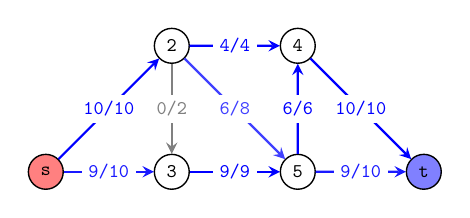
\begin{tikzpicture}[scale=0.8,every node/.style={scale=0.7},font=\tt]
	\SetUpEdge[lw         = 0.75pt,
			color      = red,
			labelcolor = white]
	\GraphInit[vstyle=Normal] 
	\SetGraphUnit{2}
	\tikzset{VertexStyle/.append  style={fill=red!50}}
	\Vertex{s}
	\tikzset{VertexStyle/.append  style={fill=white}}
	\NOEA(s){2}
	\EA(2){4}
	\tikzset{VertexStyle/.append  style={fill=blue!50}}
	\SOEA(4){t}
	\tikzset{VertexStyle/.append  style={fill=white}}
	\EA(s){3}
	\EA(3){5}
	\SetUpEdge[labeltext=blue]
	\tikzset{EdgeStyle/.style={-stealth, color=blue}}
	\Edge[label=10/10](s)(2)
	\SetUpEdge[labeltext=blue!90]
	\tikzset{EdgeStyle/.style={-stealth, color=blue!90}}
	\Edge[label=9/10](s)(3)
	\SetUpEdge[labeltext=gray]
	\tikzset{EdgeStyle/.style={-stealth, color=gray}}
	\Edge[label=0/2](2)(3)
	\SetUpEdge[labeltext=blue]
	\tikzset{EdgeStyle/.style={-stealth, color=blue}}
	\Edge[label=4/4](2)(4)
	\SetUpEdge[labeltext=blue!75]
	\tikzset{EdgeStyle/.style={-stealth, color=blue!75}}
	\Edge[label=6/8](2)(5)
	\SetUpEdge[labeltext=blue]
	\tikzset{EdgeStyle/.style={-stealth, color=blue}}
	\Edge[label=9/9](3)(5)
	\SetUpEdge[labeltext=blue]
	\tikzset{EdgeStyle/.style={-stealth, color=blue}}
	\Edge[label=10/10](4)(t)
	\SetUpEdge[labeltext=blue]
	\tikzset{EdgeStyle/.style={-stealth, color=blue}}
	\Edge[label=6/6](5)(4)
	\SetUpEdge[labeltext=blue!90]
	\tikzset{EdgeStyle/.style={-stealth, color=blue!90}}
	\Edge[label=9/10](5)(t)
\end{tikzpicture}	
\end{document}
